\section{A confidentiality-preserving approach}
\label{sec:conf}
In this paper, we present an approach for tracking and orchestrating business processes through smart contracts, conceptually in a very similar way to \cite{caterpillar},\cite{chorchain},\cite{multichain},\cite{flexchain},\cite{lorikeet},\cite{Mercenne_Brousmiche_Hamida_2018}, and \cite{Abid_Cheikhrouhou_Jmaiel_2020}, but instead of storing the process state on-chain, we apply cryptographic state commitments and accept new commitments carrying state commitment update proposals on the presentation of proper Zero-Knowledge Proofs (ZKPs). Our approach aims at rendering process state and data information undiscoverable from the smart contract state -- to parties not involved in the execution of the process instance.

ZKPs are cryptographic methods to prove that various statements are true -- without revealing any additional information about the statement. Quoting the ZKProof Community Reference (\cite{ZKProofCommunity}, p1), \emph{''A zero-knowledge proof makes it possible to prove a statement is true while preserving the confidentiality of secret information. This makes sense when the veracity of the statement is not obvious on its own, but the prover knows relevant secret information (or has a skill, like super computation ability) that enables producing proofs. The notion of secrecy is used here in the sense of prohibited leakage, but a ZKP makes sense even if the 'secret' (or any portion of it) is known apriori by the verifier(s)''}. 

In this work, we rely on zk-SNARKs, a family of \textit{noninteractive} (''single-shot'' message passing from prover to verifier), and \textit{succinct} (small and cheaply verifiable proofs) ZKPs. We use the ZoKrates toolkit as a ZKP front-end \cite{zokrates}, which currently supports the Groth16 \cite{Groth_2016} and GM17 \cite{Groth_Maller_2017} schemes.

\subsection{The zero-knowledge WorkFlow (zkWF) protocol}
Our approach relies on two key conceptual components: our zkWF (''zero knowledge WorkFlow'') protocol and what we call ''zkWF programs''.

\medskip
\noindent
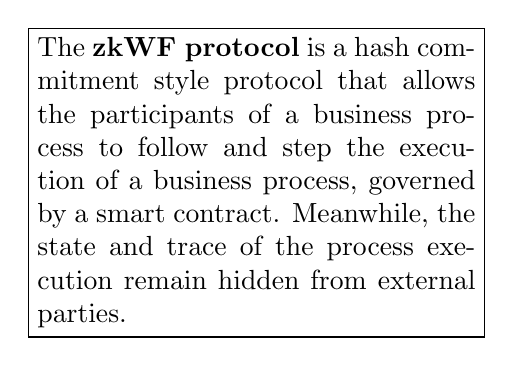
\begin{tikzpicture}
    \node[text width = \textwidth/2-0.5cm,align=justify, draw, rectangle,] {The \textbf{zkWF protocol} is a hash commitment style protocol that allows the participants of a business process to follow and step the execution of a business process, governed by a smart contract. Meanwhile, the state and trace of the process execution remain hidden from external parties.};
\end{tikzpicture}

\noindent
\section{Applications}
\label{sec:apps}
To demonstrate the wide range of usagages of our model, we implement a series of applications:
\begin{enumerate}
	\item Incremental surface \& color reconstruction
	\item 3D saliency detection
	\item Open vocabulary scene understanding
	\item Surface infrared field
	\item 3D style transfer
\end{enumerate}
Originating from our motivation in inspection and service robotics, we implement 1) Incremental surface \& color reconstruction for visualization of robot surroundings.
For robot exploration, we implement 2) 3D saliency detection to indicate the salient regions in maps.
For recovering object-level semantic information in environments, we implement 3) open vocabulary scene understanding to yield the regions containing the objects..
Furthermore, to demonstrate the flexibility, we implement 4) surface infrared fields and 5) 3D style transfer for artistic purposes. 

In~\cref{fig:latent_diff}, we classify those 3 applications into 3 categories: (a) directly obtaining the properties from sensor observation, such as application 1) and 4). (b) processing on sensor data and predict properties, such as application 2), 5). (c) extending (b) to operating beyond latent features, such as application 3).
%Thus, in the following, we discuss about those categories of applications.
% we mainly describe the application 1) (\cref{sec:incremental_reconstruction}) and 3) (\cref{sec:openvoc}).

Application 1) and 4) are in the first one category. Thus, we mainly describe 1) incremental surface \& color reconstruction (\cref{sec:incremental_reconstruction}), while for 4) we can easily exchange color with infrared.
%
For the second with 2) and 5) in~\cref{sec:fabircated_prop}, we mainly describe the usage of fabricated properties.
As the mapping part is redundant to previous category, it will not be detailed.
%
The third category is the application 3) that maps a LIM for high dimensional latent fields.
We demonstrate that this application provides a flexible inference in \cref{sec:openvoc}.


%Afterwards, we evaluate application 1) and 3) in~\cref{sec:exp} and extensively show demonstration for all application in~\cref{sec:exp:extensive_app}.


Figure \ref{fig:basic_update} presents a high-level overview of the protocol. The protocol requires to have a smart contract deployed on a blockchain for each process instance. This smart contract contains a hash commitment of the current state and an encrypted version of the state.

During process execution, the collaborating parties can send messages to each other by off-chain means. These are captured in the underlying process specification as intermediate message throw and capture events; the commitment scheme includes commitments to the message hashes.

When a participant wishes to update the state stored in the smart contract (hash commitment and state ciphertext) -- that is, to ''step the process'' --, it has to create a ZKP that the state transition they propose is valid. This new state includes the hash of the message they sent beforehand if the step involves message sending. When the execution arrives at a point where a participant receives a message in the next stage of the execution, the receiving party checks the hash and only accepts if the hashes match.

Participant authorization is tied to proving EdDSA private key ownership in the ZKPs; the public keys of the participants are defined over the underlying process model as a parameterization. Additionally, we require the participants to have a common means for encrypting and decrypting stored state ciphertexts (this aspect is not constrained by the protocol).

This scheme enables adapting the protocol to different distributed ledgers in a straightforward way (we provide an implementation for Ethereum and Hyperledger Fabric); as well as masking updater identity on pseudonymizing platforms (such as Ethereum) by facilitating the use of single-use transaction source addresses. While the updates themselves and the contract state are unintelligible to parties outside the collaboration, statistical and model trace analyses of the update sequences may still be a threat; our mitigation is the inclusion of a ''fake'' update transaction variant (no actual state update), which all participants are authorized to use freely.

\subsection{zkWF programs}
zkWF programs serve as a bridge between process specification and proof computation/verification. These programs are generated from a representative subset of the BPMN specification, with extensions for cryptographic checks, as detailed later.

\medskip
\noindent
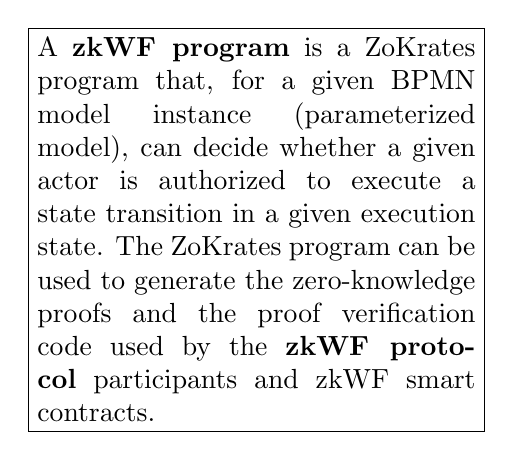
\begin{tikzpicture}
    \node[text width = \textwidth/2-0.5cm,align=justify, draw, rectangle,]{A \textbf{zkWF program} is a ZoKrates program that, for a given BPMN model instance (parameterized model), can decide whether a given actor is authorized to execute a state transition in a given execution state. The ZoKrates program can be used to generate the zero-knowledge proofs and the proof verification code used by the \textbf{zkWF protocol} participants and zkWF smart contracts.};
\end{tikzpicture}

\subsection{Toolchain overview}
We have created a prototype of an end-to-end toolchain to support the proposed approach, as depicted in figure \ref{fig:vezerabra}, from modelling through code synthesis to deployment and operation. The figure also delineates the newly created software components (and those with novel generators).

In the \textit{modelling phase}, a BPMN model is annotated with metadata for process instantiation, and our Kotlin-based interpreter and translator creates the corresponding zkWF program.

In the \textit{synthesis phase}, the ZoKrates toolkit is used to set up the \textit{prover key} and \textit{verifier key} (note that ZoKrates supports \textit{multi-party ceremonies}) and generates the verifier smart contract in Solidity. We created novel support for generating verifier code for Hyperledger Fabric \cite{hyperledger_fabric}. We also created the (necessarily application-specific) code generation facilities for the state commitment management part of the smart contracts for both platforms.

For the deployment phase, we created automation facilities for deployment to Ethereum (and other blockchains using a compatible RPC API); and an SDK and GUI application for the client side. Here we integrate the ZoKrates toolkit as a proof generator.

\noindent
\begin{figure}
	\centering
	\begin{tikzpicture}[font=\sffamily,line width=0.015cm, scale=0.5,every node/.style={scale=0.5}]
	    \node[rectangle,draw,minimum width= 3cm,minimum height=1.5cm](BPMN){BPMN};
	    \node[rectangle,draw,minimum width= 3cm,minimum height=1cm,right=0 cm of BPMN,xshift=\pgflinewidth,yshift=-0.25cm,fill=gray!20!white,xshift=-\pgflinewidth](ext){Extended attributes};
	    \node[below=0.3 cm of BPMN,xshift=-8cm,yshift=0.5cm] (m1) {};
	    \node[below=0.3 cm of ext,xshift=2.5cm,yshift=0.5cm] (m2) {};
	    \draw[dashed] (m1) -- (m2);
	    \node[above=0.5cm of m1,xshift=1cm,yshift=-1cm,draw,circle](t1){\large{I.}};
	    \node[right=0.5cm of t1,xshift=-1cm]{\large{Modelling}};
	    
	    \node[below=0.5cm of BPMN,draw,ellipse,yshift=0cm,fill=gray!20!white] (transform) {Transformation logic};
	    \draw[<-] (transform.north) -- (BPMN.south);
	    \node[below=0.5cm of transform,draw,rectangle,yshift=-0.0cm,minimum width= 3cm,minimum height=1cm,fill=gray!20!white] (zkwf) {zkWF program};
	    
	    \node[right=1.1cm of zkwf] (zokrates) {\large ZoKrates};
	    
	    \draw[<-] (zkwf.north) -- (transform.south);
	    \node[below=0.5 cm of zkwf,draw,rectangle,yshift=-0.0cm,minimum width= 3cm,minimum height=1.5cm,align=left] (keys) {prover key\\\\ verifier key};
	    \draw[<-] (keys.north) -- (zkwf.south);
	    \draw[dashed] (keys.west) -- (keys.east);
	    \node[left=0.25 cm of keys,draw,rectangle,minimum width=4.5cm,minimum height=1cm,yshift=0.375cm] (proofGen){ZoKrates proof generator};
	    \node[left=0.5cm of keys.west,xshift=1.25cm,yshift=0.375cm] (proverKeyBorder){};
	    \draw[<-] (proofGen.east) -- (proverKeyBorder);
	    \node[right=0.5 cm of keys.east,xshift=-1.25cm,yshift=-0.375cm] (verifierKeyBorder){};
	    \node[right=0.25 cm of keys,align=center,draw,rectangle,minimum width= 4.4cm,minimum height=1.75cm,yshift=-0.375cm,top color=gray!40!white, bottom color=white] (sc) {State commitment\\\&\\verifier smart contract};
	    \draw[<-] (sc.west) -- (verifierKeyBorder);
	    \draw[dashed] (sc.west) -- (sc.east);
	    \node[below=0.5cm of sc,draw,rectangle,yshift=1.0cm,minimum width=2.2cm,minimum height=1cm,xshift=-1.1cm,fill=gray!20!white,yshift=\pgflinewidth] {Java};
	    \node[below=0.5cm of sc,draw,rectangle,yshift=1.0cm,minimum width=2.2cm,minimum height=1cm,xshift=1.1cm,left color=gray!20!white, right color=white,yshift=\pgflinewidth] (solc){Solidity};
	    
	    \node[draw,rectangle,dashed, fit=(zkwf) (solc) (proofGen),minimum width=13.5cm,minimum height=5.5cm]{};
	    
	    \node[below=1.375cm of keys,xshift=-8cm] (s1) {};
	    \node[below=1.375cm of keys,xshift=6.75cm] (s2) {};
	    \draw[dashed] (s1) -- (s2);
	    \node[above=0.5cm of s1,xshift=1cm,yshift=-1cm,draw,circle](t2){\large{II.}};
	    \node[right=0.5cm of t2,xshift=-1cm]{\large{Synthesis}};
	    

	    
	    \node[below=1.75cm of keys,draw,ellipse,fill=gray!20!white,xshift=2cm] (depl) {DL specific deployment};
	    \node[below=0.1cm of sc.south,yshift=0.25cm,xshift=0.0cm] (scBot){};
	    \draw[->] (scBot) -| ++(0,-1.5) -| (depl.north); 
	    
	    \node[below=0.5cm of depl,rectangle,draw,minimum width=4.5cm,minimum height=1cm,fill=gray!20!white](sci){SC instance};
	    \draw[<-] (sci.north) -- (depl.south);
	    \node[below=0 cm of sci,rectangle,draw,minimum width=2.25cm,minimum height=1cm,yshift=\pgflinewidth,xshift=1.125cm,fill=gray!20!white,yshift=\pgflinewidth]{EVM};
	    \node[below=0 cm of sci,rectangle,draw,minimum width=2.25cm,minimum height=1cm,yshift=\pgflinewidth,xshift=-1.125cm,fill=gray!20!white,yshift=\pgflinewidth]{HL Fabric};
	    
	    \node[left=0.5cm of sci,draw,rectangle,xshift=-1.5cm,minimum width=3.85cm,minimum height=1cm,fill=gray!20!white](sdk){Participant side SDK};
	    \node[below=0cm of sdk,rectangle,draw,minimum width=3.85cm,minimum height=1cm,yshift=\pgflinewidth](web3){Web3J wallet};
	    \node[left=0.5cm of sci.south,xshift=-1cm] (sc_side){};
	    \node[right=0.5of sdk.south,xshift=0.655cm] (sdk_side){};
	    \draw[<->,line width=0.04cm] (sc_side) -- (sdk_side);
	    \node[left=0.5cm of sc_side,xshift=0.5cm,yshift=0.2cm,align=center](zkwfp){zkWF};
	    \node[below=0.0cm of zkwfp,yshift=0.1cm]{protocol};
	    \node[below=0.5 cmof web3,yshift=0.7cm,xshift=1.5cm](GUI) {WFGUI};
	    
	    \node[draw,dashed,fit=(sdk) (GUI) (web3),minimum width=4.5cm, minimum height=3cm]{};
	    
	    \node[below=0.5cm of sci,yshift=-2cm,xshift=3.5cm](note){New results*};
	    \node[draw,rectangle,fill=gray!30!white,left=0.5cm of note,xshift=1cm]{};
	    \node[below=0.2cm of note,xshift=-2cm]{*Gradients show partially new results};
	    
	    \node[below=0.5 cm of GUI,xshift=-4cm,yshift=0.5cm,draw,circle](t3){\large{III.}};
	    \node[right=0.5 cm of t3,xshift=-1cm]{\large{Deployment \& Operation}};
	\end{tikzpicture}
	\caption{Toolchain overview}
	 \label{fig:vezerabra}
\end{figure}

\subsection{Adversarial model and security goals}
A \textit{participant} of a \textit{business process instance} is a party who has a private EdDSA key necessary to enact certain state changes in the process instance, as encoded in the underlying BPMN model instance with public key annotations on model elements. All other parties are deemed \textit{process external}. 

We assume that the underlying process model is public knowledge, but the set of public keys serving as parameterization for a process instance is shared only between the participants. We also assume no private key compromises.

We assume full integrity for the blockchain (no successful attack on the consensus) but also the full observability of transactions targeting the process manager smart contract and the smart contract state sequence by process external parties. For the sake of simplicity, we assume deterministic transaction finality for the blockchain (largely equivalent to ''waiting for a few blocks'' for treating transactions as blockchain-included under probabilistic finality models). We treat the blockchain as \textit{fair} -- any transaction submitted by a participant is included in a block in a reasonable time, irrespective of concurrent transaction proposal load.

Our \textit{integrity goals} are the following.
\begin{itemize}
    \item Process external parties should not be able to influence the smart contract state commitment and stored encrypted state.
    \item Participants should be able to influence the smart contract state commitment and stored encrypted state only when they are authorized by their private key(s). Accepted state commitment updates should always conform to the execution semantics of the underlying process model.
    \item Should a participant successfully submit an encrypted state not conforming to the accompanying commitment, it has to be evident to all participants in a non-repudiable way.
\end{itemize}

The first two integrity goals largely carry over from the earlier cited state of the art; the third is a reasonable relaxation in view of a currently still missing ZKP capability, as explained later.

Our \textit{availability goal} is that no process external party should be able to influence the update capability of the authorized participants.

Lastly, our \textit{confidentiality goal} is that no external party should be able to determine the process state either fully or partially (beyond the fact that it exists and that it has been started) without collusion with at least one participant.


%is key-authorized process state changes to be possible only in terms of the smart contract state commitment and stored encrypted state. 
%Note that this goal carries over from the existing state of the art.

%Our \textit{availability goal} is no process external party to stop

%In this paper, we assume the following properties may apply for a given attacker:


%\begin{itemize}
%\item An attacker knows the corresponding BPMN model for a given smart contract instance
%\item A malicious participant may also be an attacker
%\end{itemize}

%Our approach aims at ensuring the following security guarantees.
%\todo{Ezeket befelyezni}
%\begin{itemize}  
% \item Parties not participating cannot modify the state stored on the blockchain
% \item Parties not participating cannot read or guess the current state of the business process execution based on the data stored in the smart contract. 
%\item No party can make an illegal move during the orchestration.
%\item Messages between the participants can be verified.
%\item Participants can identify which party made a given move 
%\end{itemize}